\documentclass[12pt]{article}
\usepackage{float}
\usepackage[margin=0.8in]{geometry}
\usepackage[utf8]{inputenc}
\usepackage[fleqn]{amsmath}
\usepackage{times}
\usepackage{graphicx}
\usepackage{mathptmx}
\usepackage[font=scriptsize,labelfont=bf]{caption}
\graphicspath{{./img/}}

\title{CS3211 Project 1}
\author{Tan Soon Jin, A0112213E \\ a0112213@u.nus.edu}
\date{\today}

\begin{document}
\maketitle
\section*{Part 1}

\subsection*{Hardware}

  \begin{table}[H]
    \centering
    \begin{tabular}{|l|l|l|l|l|l|l|}
      \hline
      Machines
    & \begin{tabular}[c]{@{}l@{}}Number\\ of cores\end{tabular} &
    \begin{tabular}[c]{@{}l@{}}Clock Speed\\ (GHz)\end{tabular} &
    \begin{tabular}[c]{@{}l@{}}Total Memory\\ (GB)\end{tabular} &
    \begin{tabular}[c]{@{}l@{}}L1 cache\\ (kB)\end{tabular} &
    \begin{tabular}[c]{@{}l@{}}L2 cache\\ (kB)\end{tabular} &
    \begin{tabular}[c]{@{}l@{}}L3 cache\\ (kB)\end{tabular} \\ \hline
    \begin{tabular}[c]{@{}l@{}}CS3211 Lab\\ Intel i7-2600\end{tabular}
      & 8                                                         & 3.4
      & 16                                                          & 64
      & 256                                                     & 8192
      \\ \hline
      \begin{tabular}[c]{@{}l@{}}Tembusu Cluster\\ Intel Xeon
      E5-2620\end{tabular} & 24
      & 2.4                                                         & 64
      & 64                                                      & 256
      & 15260                                                   \\ \hline
    \end{tabular}
    \caption{Hardware specifications}
    \label{fig:hardware}
  \end{table}
  
  \begin{enumerate}
    \item For program that does not utilize parallelization, lab machine
      with higher clock speed outperforms Tembusu machine (task 1).
    \item Tembusu machine with more cores allow for better distribution
      of workload is able to complete the matrix multiplication under
      shorter time.
  \end{enumerate}

\subsection*{Lab1: Speedup}

  \subsubsection*{Task 3}
    \begin{figure}[ht]
      \centering
      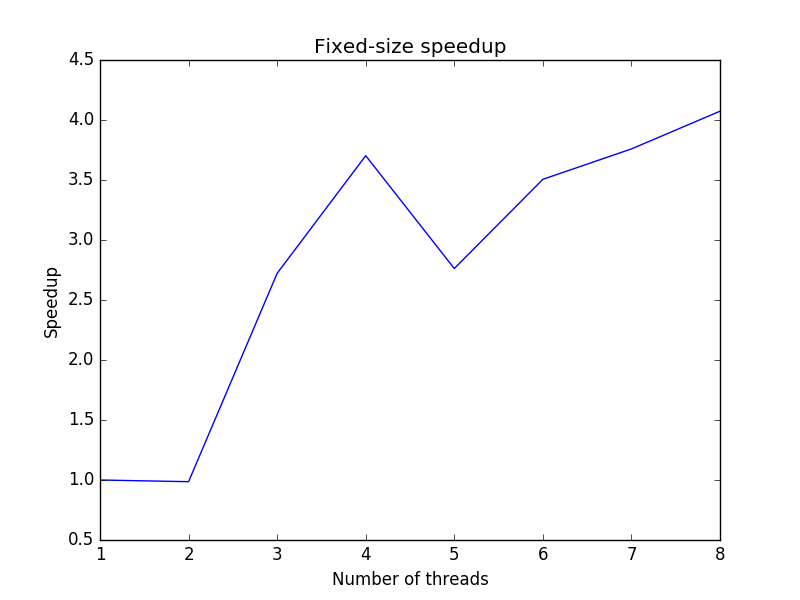
\includegraphics[width=0.45\linewidth]{lab1_task3_fixedsize}\hfill
      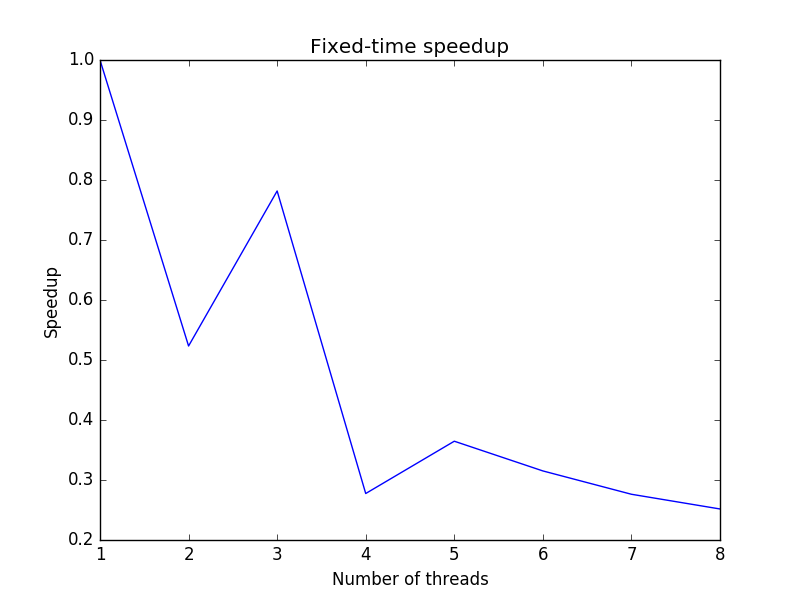
\includegraphics[width=0.45\linewidth]{lab1_task3_fixedtime}
      \caption{Comparing Fixed-size speedup and Fixed-time speedup}
      \label{fig:task3_speedup}
    \end{figure}
    \newpage

  \subsubsection*{Task 4}
    \begin{figure}[ht]
      \centering
      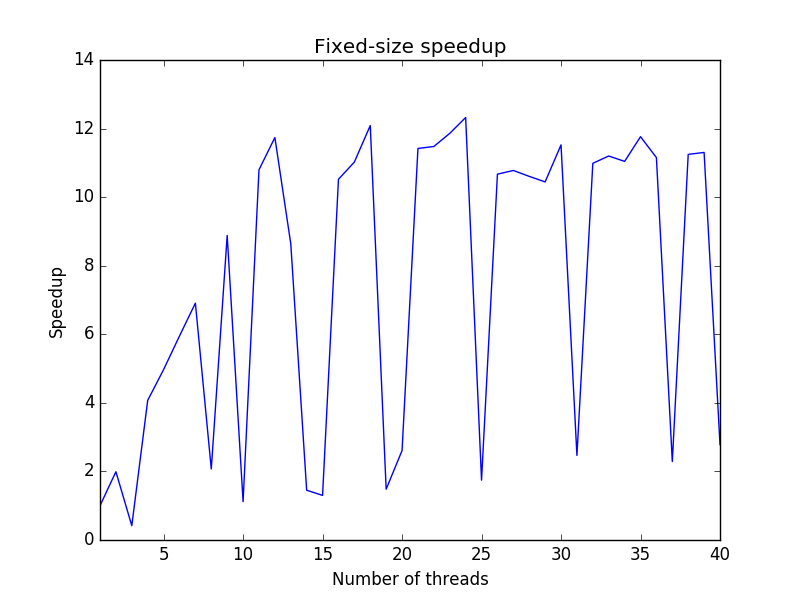
\includegraphics[width=0.45\linewidth]{lab1_task4_fixedsize}\hfill
      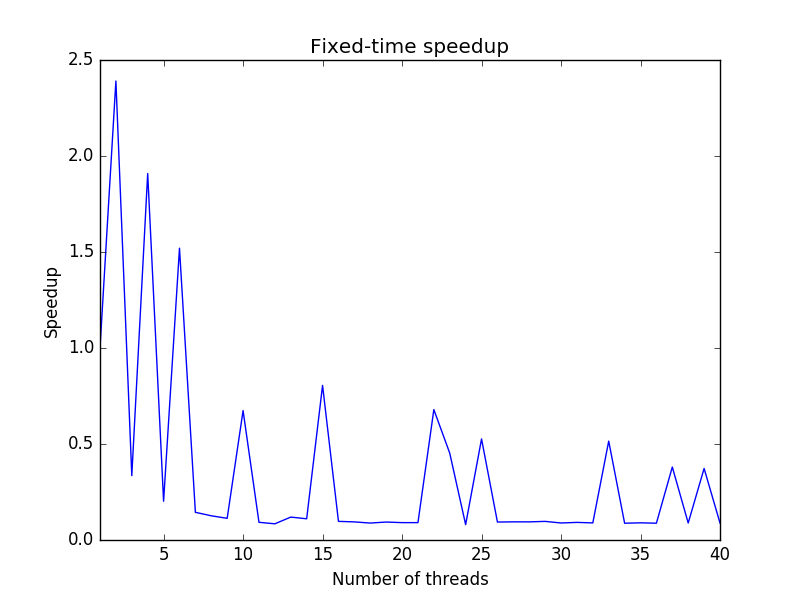
\includegraphics[width=0.45\linewidth]{lab1_task4_fixedtime}
      \caption{Comparing Fixed-size speedup and Fixed-time speedup}
      \label{fig:task4_speedup}
    \end{figure}

\subsection*{Lab1: Memory effects}

  \subsubsection*{Task 6}
    \begin{figure}[ht]
      \centering
      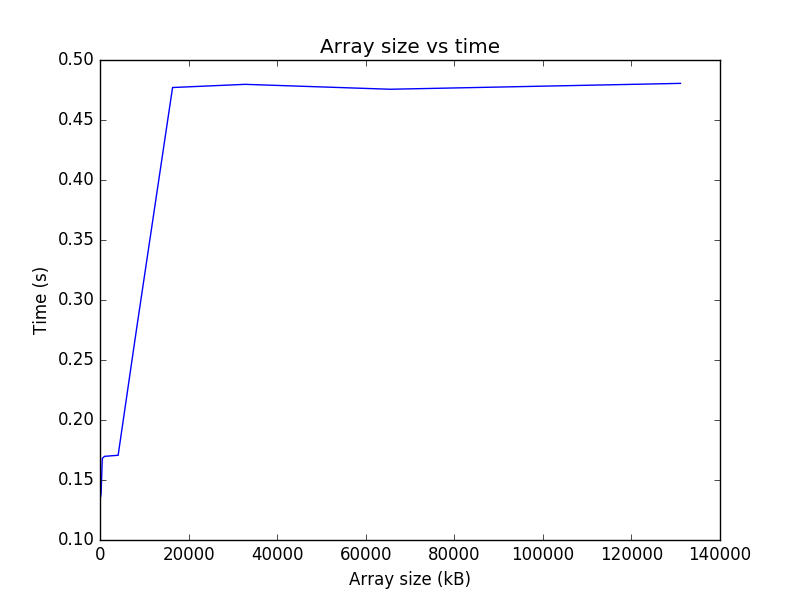
\includegraphics[width=0.5\linewidth]{lab1_task6}
      \caption{Relationship between array size and time}
      \label{fig:task6_memory}
    \end{figure}

\subsection*{Lab 2: Accuracy}

  \subsubsection*{Task 1}
  \begin{table}[H]
    \centering
    \begin{tabular}{|l|l|}
      \hline
      Number of 1s & Sum        \\ \hline
      500000       & 500000.0   \\ \hline
      1000000      & 1000000.0  \\ \hline
      18000000     & 16777216.0 \\ \hline
      18500000     & 16777216.0 \\ \hline
      19000000     & 16777216.0 \\ \hline
      19500000     & 16777216.0 \\ \hline
    \end{tabular}
    \caption{Adding 1 to 0 accuracy problem}
    \label{fig:lab2_task1}
  \end{table}

  \subsubsection*{Task 2}
  \begin{table}[H]
    \centering
    \begin{tabular}{|l|l|}
      \hline
      Number of 1s & Sum       \\ \hline
      500000       & 500000.3  \\ \hline
      1500000      & 1500000.2 \\ \hline
      3500000      & 3500000.2 \\ \hline
      4000000      & 4000000.2 \\ \hline
      6000000      & 6000000.0 \\ \hline
      6500000      & 6500000.0 \\ \hline
      7000000      & 7000000.0 \\ \hline
      7500000      & 7500000.0 \\ \hline
      9500000      & 9500000.0 \\ \hline
    \end{tabular}
    \caption{Adding 1 to 0.3 accuracy problem}
    \label{fig:lab2_task2}
  \end{table}

  \subsubsection*{Task 3}
  \begin{table}[H]
    \centering
    \begin{tabular}{|l|l|}
      \hline
      Order            & Sum        \\ \hline
      Sum from 20 to 1 & 584.660156 \\ \hline
      Sum from 1 to 20 & 584.660156 \\ \hline
    \end{tabular}
    \caption{Adding pseudo random numbers in different orders}
    \label{fig:lab2_task3}
  \end{table}

  \subsubsection*{Task 4}
  \begin{table}[H]
    \centering
    \begin{tabular}{|l|l|}
      \hline
      Trial & Sum            \\ \hline
      1     & 3056623.750000 \\ \hline
      2     & 3056623.750000 \\ \hline
      3     & 3056623.750000 \\ \hline
      4     & 3056623.750000 \\ \hline
      5     & 3056623.750000 \\ \hline
      6     & 3057561.000000 \\ \hline
      7     & 3057560.750000 \\ \hline
      8     & 3057560.750000 \\ \hline
      9     & 3057561.000000 \\ \hline
      10    & 3057561.000000 \\ \hline
    \end{tabular}
    \caption{Adding 10000 psudo random numbers using 24 threads}
    \label{fig:lab2_task4}
  \end{table}

\subsection*{Lab 2: Communication, speedup}
  
  \subsubsection*{Task 7}
    \begin{figure}[ht]
      \centering
      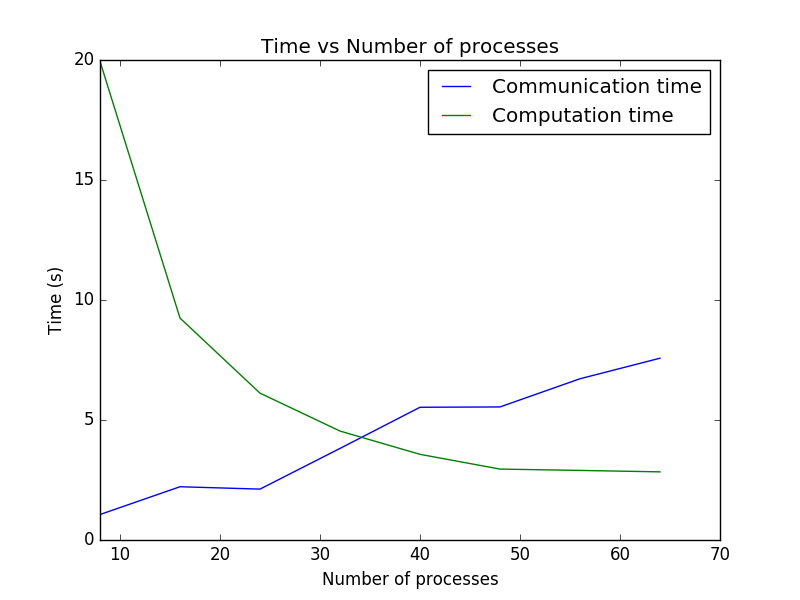
\includegraphics[width=0.5\linewidth]{lab2_task7}
      \caption{Number of processes vs Communication time and Computation
      time}
      \label{fig:lab2_task7}
    \end{figure}


\section{Part 2}

\subsection{Tabulation}
\subsection{Discussion}
\subsection{Conclusion}
\end{document}
